\documentclass{beamer}
\usefonttheme{serif}
\usepackage[T1]{fontenc}
\usepackage[spanish,es-tabla]{babel}
\uselanguage{Spanish}
\languagepath{Spanish}
%%%% No estamos usando realmente bibliografía, pero si no incluimos
%    este paquete, no funciona la compilación con makefile.
\usepackage[backend=biber, style=apa, citestyle=apa]{biblatex}
\addbibresource{bibliography/sources.bib}
%%%%%%%%
\usetheme{Madrid}
\usepackage{xcolor}
    \definecolor{gray}{rgb}{0.5,0.5,0.5}
    \definecolor{lightYellow}{RGB}{251, 255, 212}
    \definecolor{lightBlue}{RGB}{56,184,255}
\usepackage{listings}
\renewcommand{\lstlistingname}{Programa}
\lstset{
    basicstyle=\ttfamily\footnotesize,
    numberstyle=\ttfamily,
    xleftmargin=2em,
    frame=rlbt, % draw a frame at the top and bottom of the code block
    tabsize=4, % tab space width
    showstringspaces=false, % don't mark spaces in strings
    numbers=left, % display line numbers on the left
    commentstyle=\color{gray}, % comment color
    keywordstyle=\color{blue}, % keyword color
    stringstyle=\color{red}, % string color
    backgroundcolor=\color{lightYellow},
    captionpos=b,
    breaklines=true,
    literate=
            {Á}{{\'{A}}}1
            {É}{{\'{E}}}1
            {Í}{{\'{I}}}1
            {Ó}{{\'{O}}}1
            {Ú}{{\'{U}}}1
            {á}{{\'{a}}}1
            {é}{{\'{e}}}1
            {í}{{\'{i}}}1
            {ó}{{\'{o}}}1
            {ú}{{\'{u}}}1
            {ñ}{{\~{n}}}1
            {Ñ}{{\~{N}}}1
            {ü}{{\"{u}}}1
            {Ü}{{\"{U}}}1
            {¡}{{!`}}1
            {¿}{{?`}}1
}
%\usecolortheme{beaver}
\graphicspath{{img/}}
\author[Rodríguez y Brown]{
    Francisco Rodríguez Melgar\inst{1}\\
    Dr. Emmett Lathrop Brown\inst{2}\\
}
\title[Ejemplo beamer]{
    Ejemplo de presentación con \LaTeX{}
}
\subtitle{
    Cómo hacer presentaciones con \LaTeX{} y Beamer
}
\institute[UdE y Caltech]{
    \inst{1}Universidad de Ejemplo \\
    Facultad de las cosas que molan\and
    \inst{2}Instituto Tecnológico de California\\
    Facultad de Viajes en el Tiempo

}
\date[Esp. Conf.]{
    Conferencias Espaciales -- \today
}
\begin{document}
    \begin{frame}
        \titlepage
    \end{frame}
    \begin{frame}
        \frametitle{Contenido}
        \tableofcontents
    \end{frame}
    \section{Introducción}
    \begin{frame}
        \frametitle{Introducción}
        Esta presentación quiere cumplir una función parecida a la del
        documento principal del tutorial, será una pequeña presentación de
        transparencias en las que se podrá ver el código y el resultado
        para entender cómo se hacen las cosas que aparecen aquí.
    \end{frame}
    \section{Transparencias simples}
    \begin{frame}
        \frametitle{Transparencia simple}
        En las transparencias (entornos \textit{frame}) el texto que se incluya
        se incluirá centrado horizontal y verticalmente. Del mismo modo que
        en cualquier párrafo de texto se pueden usar los comandos de formato,
        tanto \textit{itálica} como \textbf{negrita}.
    \end{frame}
    \begin{frame}
        \frametitle{Listas numeradas y sin numerar}
        Es muy sencillo crear listas numeradas o sin numerar, que se
        formatearán de manera sencilla junto con el resto de párrafos. Por
        ejemplo, en estas transparencias ya hemos visto:
        \begin{itemize}
            \item Cómo introducir texto.
            \item Cómo formatear ese texto.
            \item Cómo ponerle títulos a las transparencias.
        \end{itemize}
        Aún nos queda por ver:
        \begin{enumerate}
            \item Cómo crear transparencias a dos -o más- columnas.
            \item Cómo introducir ecuaciones.
            \item Cómo introducir figuras.
            \item Cómo introducir bloques especiales.
        \end{enumerate}
    \end{frame}
    \section{Transparencias avanzadas}
    \begin{frame}
        \frametitle{Transparencias a dos columnas}
        \begin{columns}
            \begin{column}{.5\hsize}
                Esta es una transparencia a dos columnas, suelen ser útiles para
                establecer paralelismos, por ejemplo, podemos comparar un
                párrafo con el mismo en negrita. 
            \end{column}
            \begin{column}{.5\hsize}
                \textbf{Esta es una transparencia a dos columnas,
                suelen ser útiles para
                establecer paralelismos, por ejemplo, podemos comparar un
                párrafo con el mismo en negrita.}
            \end{column}
        \end{columns}
    \end{frame}
    \begin{frame}
        \frametitle{Introducción de imágenes}
        Las imágenes se introducen como en los documentos normales, dentro de
        una figura.
        \begin{figure}[H]
            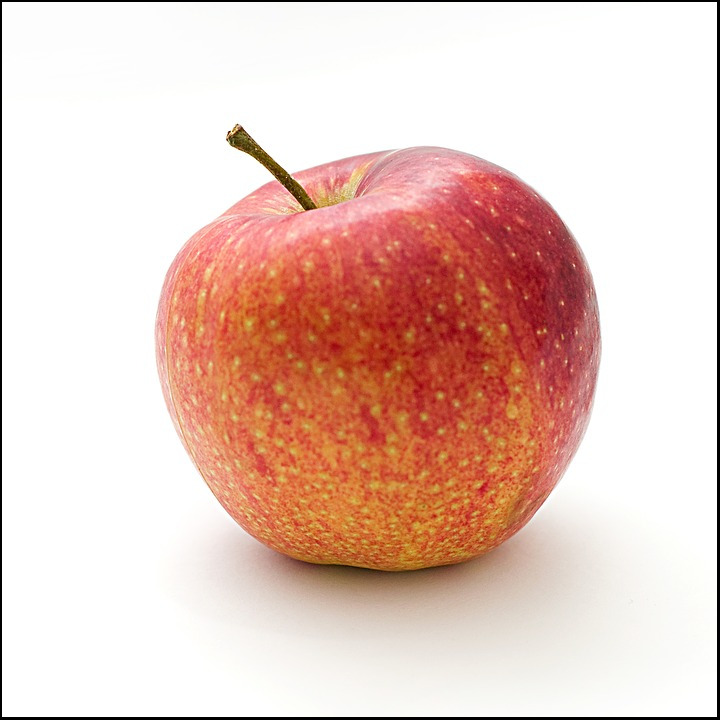
\includegraphics[width=.3333\hsize]{manzana}
            \caption{Una manzana}
            \label{fig:manzana}
        \end{figure}
        Aunque hay que tener cuidado, el contenido puede desbordarse fácilmente.
    \end{frame}
    \begin{frame}
        \frametitle{Figura y dos columnas}
        Otro de los usos más comunes de una transparencia a dos columnas es
        introducir un texto y una figura a su lado:
        \begin{columns}
            \begin{column}{.5\hsize}
                El gato doméstico (nombre científico:
                \textit{Felis silvestris catus})
                es un mamífero del la subfamilia de los felinos que ha
                desarrollado una relación de domesticación con el ser humano.
                La raza más común es el gato de pelo corto europeo, como el
                de la figura.
            \end{column}
            \begin{column}{.5\hsize}
                \begin{figure}[H]
                    
\includegraphics[width=.75\hsize]{gatito}
                    \caption{Un gatito blanco}
                    \label{fig:gatito}
                \end{figure}
            \end{column}
        \end{columns}
    \end{frame}
    \begin{frame}
        \frametitle{Ecuaciones}
        Como se ha dicho en el documento principal del tutorial, las
        ecuaciones en la clase \textit{beamer} se deben incluir con la notación
        <<moderna>>, compatible con el paquete \texttt{amsmath}.
    \end{frame}
    \begin{frame}
        \frametitle{Bloques especiales}
        \begin{block}{El Binomio de Newton}
            \[
                (a+b)^{n}=\sum_{i=-1}^{n}
                {
                    \begin{pmatrix}
                        n \cr i
                    \end{pmatrix} a^{n-i}b^{i}
                }
            \]
        \end{block}
        \begin{alertblock}{Cuidado}
            \centering
            \(n \in \mathbb{N} \), y cuidado con el signo de \(a\) y \(b\).
        \end{alertblock}
        \begin{examples}
            \[
                (3x+y)^{2} = 9x^2+6xy+y^2
            \]
        \end{examples}
    \end{frame}
    \section{Bloques especiales}
    \begin{frame}
        \frametitle{Bloques especiales}
        Hay que tener cuidado, el entorno \textit{frame} no permite introducir
        entornos \texttt{verbatim} de ningún tipo, ni \textit{inline} ni en
        bloque, por lo que si se desea utilizar uno, debe hacerse incluyendo
        la opción \texttt{fragile} en la orden \textit{begin}.
    \end{frame}
    \begin{frame}[fragile]
        \frametitle{Bloque verbatim}
        \begin{verbatim}
#include <stdio.h>
#include <stdlib.h>
#include <stdint.h>
int main(int argc, const char* argv[])
{
    const uint16_t MAX_NAME_SIZE = 1024;
    char* nombre = malloc(sizeof(char) * MAX_NAME_SIZE);
    printf("Dime tu nombre y pulsa [ENTER]\n");
    scanf("%s", nombre);
    printf("¡Hola, %s!\n", nombre);
    return EXIT_SUCCESS;
}
        \end{verbatim}
    \end{frame}
    \begin{frame}[fragile, containsverbatim]
        \frametitle{Bloque \texttt{lstlisting}}
        Al igual que en los documentos <<normales>>, podemos querer usar bloques
        de código con mejor estilo. De nuevo, hay que poner la opción
        \texttt{fragile}.
        
        \begin{lstlisting}[ language={C}, label={lst:holaMundo},
                            caption={Hola Mundo en C}, frame=single ]
#include <stdio.h>
#include <stdlib.h>
#include <stdint.h>
int main(int argc, const char* argv[])
{
    const uint16_t MAX_NAME_SIZE = 1024;
    char* nombre = malloc(sizeof(char) * MAX_NAME_SIZE);
    printf("Dime tu nombre y pulsa [ENTER]\n");
    scanf("%s", nombre);
    printf("¡Hola, %s!\n", nombre);
    return EXIT_SUCCESS;
}
        \end{lstlisting}
    \end{frame}
    \begin{frame}[fragile]
        \frametitle{Bloque \texttt{lstlisting} II}
        Hay que tener cuidado con una cosa, hay que añadir la opción
        \verb!xleftmargin! en nuestro bloque \verb!lstset!. Por ejemplo a
        \verb!2em!, si no, los números de línea saldrían fuera del párrafo.
        Además, es recomendable añadir \verb!\tiny! al estilo para que el texto
        sea un poco más pequeño. Si se busca en el código de esta presentación
        el bloque \verb!lstset!, se verán las órdenes modificadas.
    \end{frame}
    \section{Sobre la bibliografía}
    \begin{frame}
        \frametitle{Citas}
        Del mismo modo que se utiliza bibliografía en otro documentos, se
        puede utilizar en presentaciones de transparencias. Se puede citar y se
        puede incluir bibliografía de la misma manera. Por ejemplo:
        <<El lenguaje C++ es un superconjunto del lenguaje C>>(\cite{cpppl})
        Y, en la siguiente transparencia, podemos incluir la bibliografía.
    \end{frame}
    \begin{frame}
        \frametitle{Bibliografía}
        \printbibliography
    \end{frame}
\end{document}
